% Self-contained Overleaf source. Place this file and reports/figures/ in one project.
\documentclass[sigconf]{acmart}
\setcopyright{none}
\settopmatter{printacmref=false}
\renewcommand\footnotetextcopyrightpermission[1]{}
\acmConference{Solar Filament Segmentation Challenge 2026}{}{2026}

\usepackage[T1]{fontenc}
\usepackage{xcolor}
\usepackage{graphicx}
\usepackage{booktabs}
\usepackage{tabularx}
\usepackage{amsmath}
\usepackage{tikz}
\usetikzlibrary{positioning,arrows.meta}
\hypersetup{colorlinks=true,linkcolor=blue,urlcolor=blue,citecolor=blue}

\begin{document}

\title{A Multi-Model Instance Segmentation Pipeline for Solar Filaments}
\subtitle{A Solution to the Solar Filament Segmentation Challenge 2026}

\author{Harshit Ravindra Kulkarni}
\affiliation{\institution{SRM Institute of Science and Technology}\city{Chennai}\country{India}}
\email{kulharshit21@gmail.com}

\begin{abstract}
We present a reproducible instance-segmentation system for the Solar Filament Segmentation Challenge 2026. The method combines YOLO11x-seg proposals, Mask2Former global masks, and SAM 2.1 boundary refinement. Date-grouped validation, rater-aware targets, out-of-fold selector calibration, confidence and area filtering, and disjoint-mask arbitration are used to optimize Panoptic Quality. The preserved final CSV contains 1,261 predicted instances across 180 test images and achieved a public Kaggle score of 0.40.
\end{abstract}

\maketitle

\section{Introduction}
The challenge requires one segmentation mask for every predicted solar filament in each 2048$\times$2048 GONG H-alpha image \cite{competition}. Predictions are scored by Panoptic Quality (PQ), which jointly penalizes poor mask overlap, false detections, missed filaments, over-merging, and fragmentation. Consequently, maximizing detector recall alone is insufficient: a successful system must preserve thin morphology while rejecting uncertain candidates.

Our solution uses complementary local and global segmentation models followed by an out-of-fold calibrated instance selector. The released artifact preserves the exact 0.40 public-score submission rather than replacing it with later unscored reconstructions.

\section{Data Preparation and Model Architecture}
\subsection{Training data and split design}
The official MAGFiLO JSON annotations were parsed while retaining individual rater views. Images were grouped by observation date before fold assignment, preventing nearby observations from leaking across the train-validation boundary. Only official training images and annotations were used for training and calibration. Test images were used only for final inference.

H-alpha images were processed deterministically: grayscale conversion, intensity normalization, and contrast-limited adaptive histogram equalization (CLAHE). The same image preparation path was used for train and test inference. Training-only area statistics defined the minimum-area threshold.

\subsection{Three-model ensemble}
YOLO11x-seg produces high-recall local instance proposals. Mask2Former with a COCO-initialized Swin-Large backbone supplies global context for long and low-contrast structures. SAM 2.1 Hiera-L refines box-prompted candidate boundaries. The three components have different failure modes, so fusion is preferable to relying on a single segmentation source.

\begin{figure}[t]
\centering
\resizebox{\columnwidth}{!}{
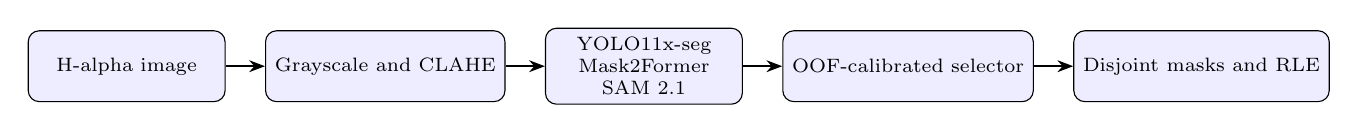
\begin{tikzpicture}[
box/.style={draw,rounded corners,align=center,font=\scriptsize,minimum width=25mm,minimum height=9mm,fill=blue!7},
arrow/.style={-{Stealth[length=2mm]},thick}]
\node[box] (i) {H-alpha image};
\node[box,right=5mm of i] (p) {Grayscale and CLAHE};
\node[box,right=5mm of p] (m) {YOLO11x-seg\\Mask2Former\\SAM 2.1};
\node[box,right=5mm of m] (s) {OOF-calibrated selector};
\node[box,right=5mm of s] (r) {Disjoint masks and RLE};
\draw[arrow] (i)--(p); \draw[arrow] (p)--(m); \draw[arrow] (m)--(s); \draw[arrow] (s)--(r);
\end{tikzpicture}}
\caption{End-to-end data flow from H-alpha image to submission CSV.}
\label{fig:pipeline}
\end{figure}

\clearpage
\section{Training, Fusion, and Qualitative Outputs}
\subsection{Training procedure}
YOLO11x-seg was trained as the high-resolution proposal model. Mask2Former was initialized from a COCO-pretrained checkpoint and fine-tuned for filament segmentation using mixed precision and distinct backbone/decoder learning rates. The SAM 2.1 image encoder was kept frozen while its decoder was used for candidate-boundary refinement. Distributed training used date-grouped folds and periodic organizer-aligned PQ validation.

\subsection{Out-of-fold candidate selection}
The selector was tuned only on out-of-fold predictions. Candidate masks were filtered by confidence and by training-derived area bounds, then duplicate or overlapping predictions were resolved through deterministic pixel arbitration. This prevents a single pixel from being assigned to multiple final instances.

\begin{table}[t]
\centering
\caption{Recovered final selector policy.}
\begin{tabular}{ll}
\toprule
Parameter & Value \\
\midrule
Fusion family & YOLO-family + Mask2Former \\
Fusion weight & 1:1 \\
Mask threshold & 0.45 \\
Score threshold & 0.53 \\
Minimum area & 319 pixels \\
Maximum area & 70,502 pixels \\
CRF refinement & Disabled \\
Overlap policy & Disjoint pixel arbitration \\
Output & COCO RLE \\
\bottomrule
\end{tabular}
\label{tab:policy}
\end{table}

\begin{figure}[t]
\centering
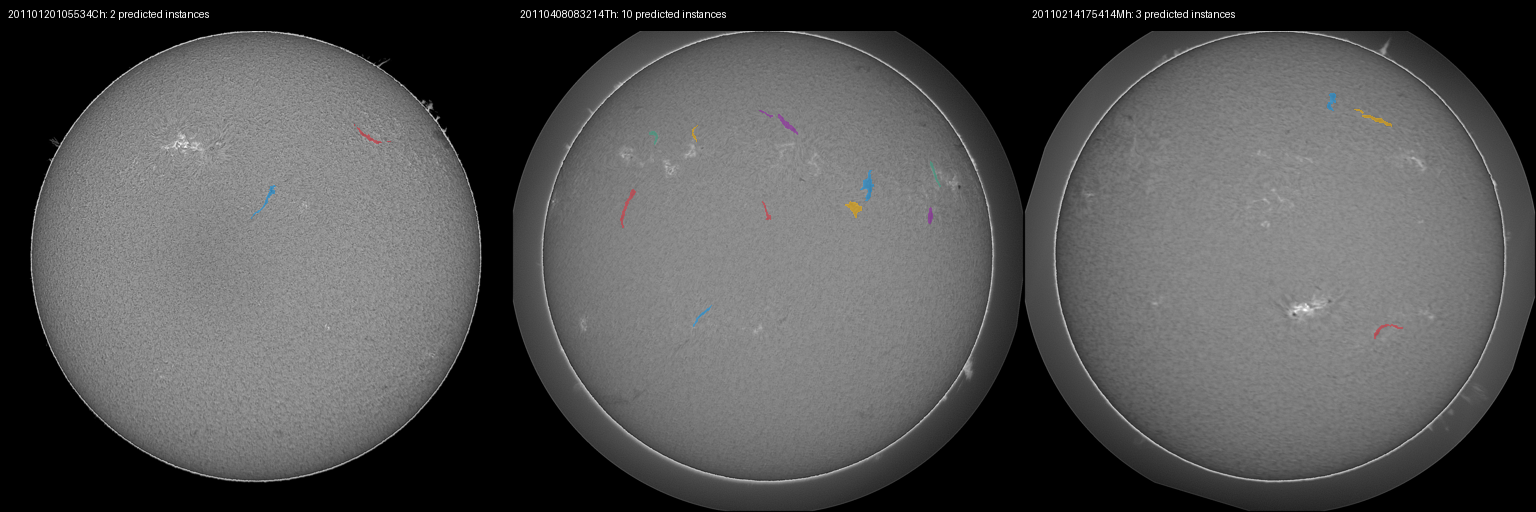
\includegraphics[width=\columnwidth]{figures/qualitative_predictions.png}
\caption{Representative test-image overlays from the exact verified 0.40 submission. Colored regions are individual predicted filament masks. These examples are qualitative illustrations only; test labels are not available locally.}
\label{fig:qualitative}
\end{figure}

The qualitative examples in Figure~\ref{fig:qualitative} show separated masks over full-disk H-alpha images. The final RLE encoder verifies image coverage, unique instance identifiers, RLE decodability, and zero overlapping output pixels before writing the submission file.

\section{Evaluation}
\subsection{Metric and protocol}
The official score is Panoptic Quality:
\[
\mathrm{PQ}=\frac{\sum_{(y,\hat y)\in TP}\mathrm{IoU}(y,\hat y)}{|TP|+0.5|FP|+0.5|FN|}.
\]
A prediction is a true positive only when it matches a human-annotated instance at IoU $\geq 0.50$. Therefore, false positives and false negatives are directly penalized, while segmentation quality among matched objects is captured by Segmentation Quality (SQ). Recognition Quality (RQ) captures the detection component.

\begin{table}[t]
\centering
\caption{Out-of-fold evaluation and final submission integrity.}
\begin{tabular}{lr}
\toprule
Measure & Value \\
\midrule
OOF PQ & 0.4622 \\
OOF SQ & 0.6857 \\
OOF RQ & 0.6741 \\
True positives / false positives / false negatives & 1031 / 454 / 543 \\
Test images & 180 \\
Final submission instances & 1,261 \\
Output overlap pixels & 0 \\
Undecodable RLEs & 0 \\
Public Kaggle score & 0.40 \\
\bottomrule
\end{tabular}
\label{tab:metrics}
\end{table}

\begin{figure}[t]
\centering
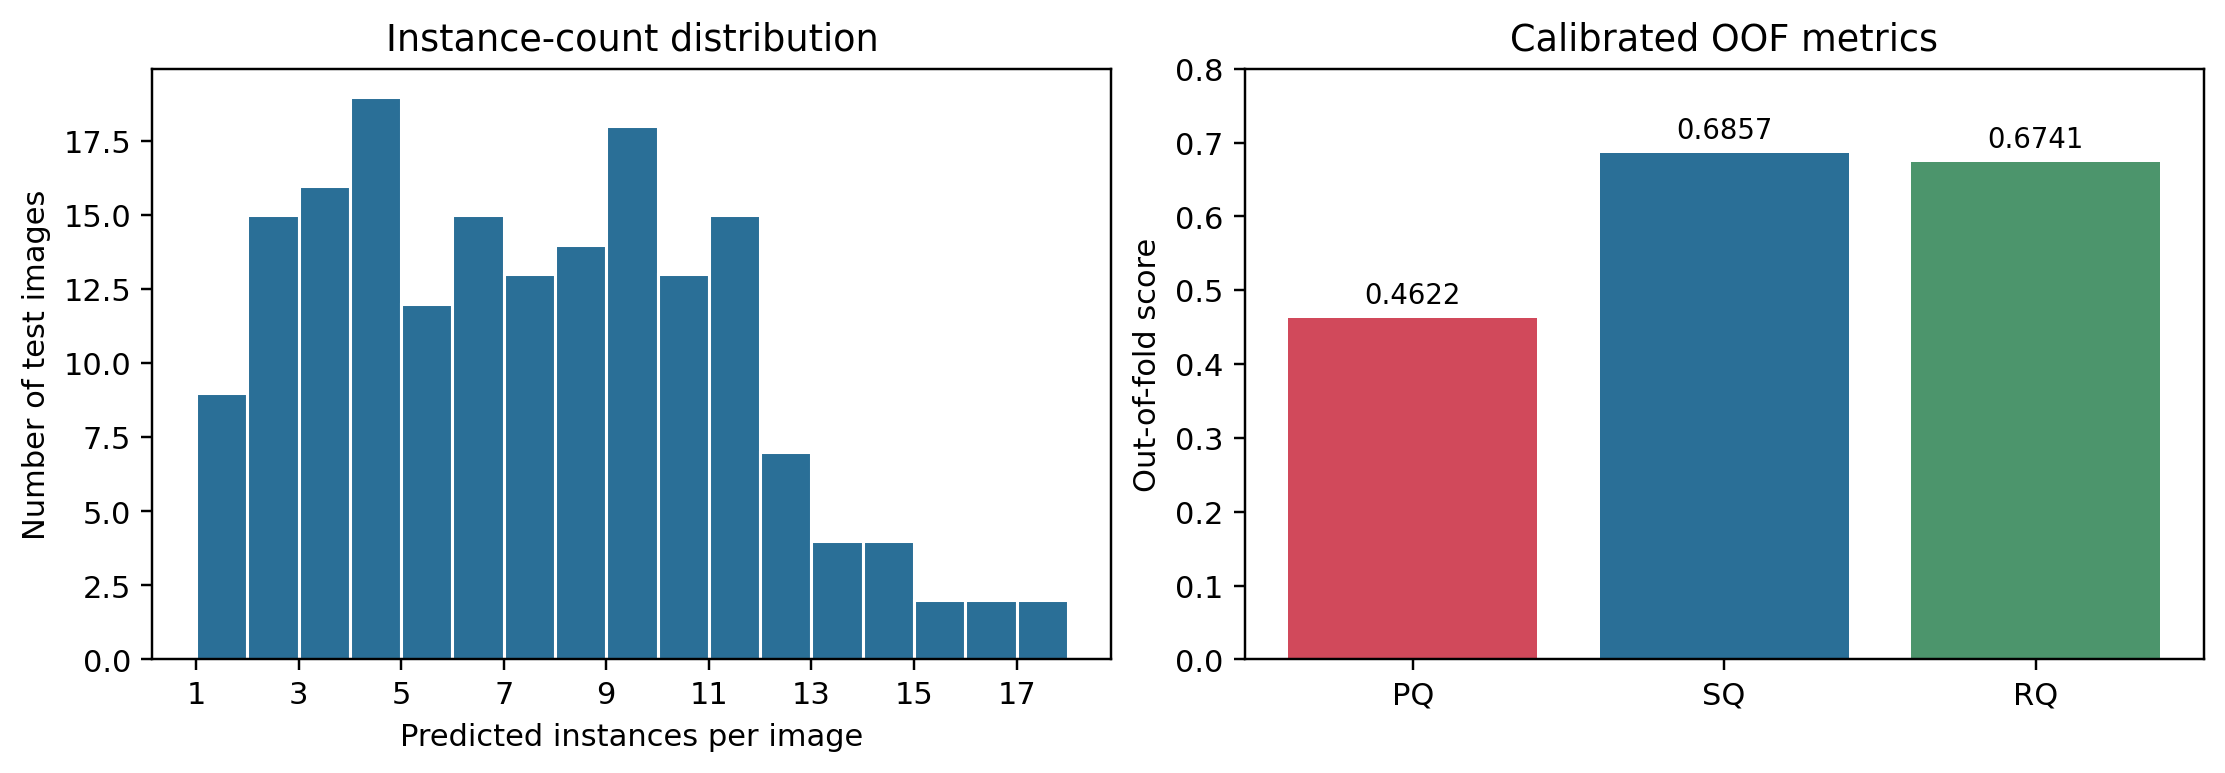
\includegraphics[width=\columnwidth]{figures/submission_distribution.png}
\caption{Submission instance-count distribution and calibrated OOF metrics. No test-set uncertainty estimate is reported because test labels are hidden.}
\label{fig:metrics}
\end{figure}

The exact final CSV has SHA-256 hash \texttt{4ee79cb588f9415eb2f48ebb1a129382f0d7f5e6410724be8b9f6b213b18e512}. It contains 1,261 rows across 180 test images. The known-good file is preserved unchanged and is distinct from a later local regeneration, which produced 1,147 rows and was intentionally not submitted.

\clearpage
\section{Strengths, Limitations, and Reproducibility}
The ensemble benefits from complementary model behavior. YOLO11x-seg identifies narrow local candidates; Mask2Former supplies global context for extended or ambiguous structures; SAM refinement preserves local boundaries. Conservative calibration and disjoint arbitration reduce duplicate detections and structural errors.

The principal limitation is that original blind-test prediction caches from the historical run were not retained. Re-running recovered model weights on a later machine produced a valid but non-identical CSV. To preserve submission integrity, the exact known-good 0.40 file remains the final artifact.

The public release contains source code, configurations, requirements, verification scripts, a Kaggle runner, figure-generation scripts, and integrity documentation. The weights and exact CSV are hosted separately to avoid putting large binaries or competition artifacts directly into source control.

\begin{itemize}
\item Code: \url{https://github.com/kulharshit21/solar-filament-final-draft}
\item Weights and exact submission: \url{https://drive.google.com/open?id=1qikTNZkhUWEC3vB0Yz2_5l5Zwr1AehFN}
\item Canonical CSV: \texttt{submission\_040\_verified.csv}
\end{itemize}

All training, calibration, and inference decisions described here use only permitted competition data. No hidden labels, organizer evaluation outputs, credentials, or prohibited metadata are included in the release.

\clearpage
\section{Acknowledgment}
The organization of the Filament Segmentation Challenge 2026 is partially supported by the U.S. National Science Foundation (NSF) under Grant No. 2209912 and 2433781, directorate for Computer and Information Science and Engineering (CSE), and Office of Advanced Cyberinfrastructure (OAC), and Grant No. 2511630, AST Division Of Mathematical and Physical Sciences.

The Filament Segmentation Challenge 2026 is sponsored by the U.S. National Science Foundation (NSF) National Solar Observatory (NSO).

This work utilizes GONG data obtained by the NSO Integrated Synoptic Program, managed by the National Solar Observatory, which is operated by the Association of Universities for Research in Astronomy (AURA), Inc. under a cooperative agreement with the National Science Foundation and with contribution from the National Oceanic and Atmospheric Administration. The GONG network of instruments is hosted by the Big Bear Solar Observatory, High Altitude Observatory, Learmonth Solar Observatory, Udaipur Solar Observatory, Instituto de Astrofísica de Canarias, and Cerro Tololo Interamerican Observatory.

\begin{thebibliography}{9}
\bibitem{competition} A. Ahmadzadeh, D. J. Kempton, Q. Li, and A. A. Pevtsov. Solar Filament Segmentation Challenge 2026. \url{https://www.kaggle.com/competitions/filament-segmentation-2026}, 2026.
\bibitem{magfilo} A. Ahmadzadeh et al. MAGFiLO: Manually Annotated GONG Filaments from H-alpha Observations. \textit{Scientific Data}, 2024. doi: \url{https://doi.org/10.1038/s41597-024-03876-y}.
\bibitem{mask2former} B. Cheng et al. Masked-attention Mask Transformer for Universal Image Segmentation. \textit{Proceedings of CVPR}, 2022.
\bibitem{sam} A. Kirillov et al. Segment Anything. \textit{Proceedings of ICCV}, 2023.
\end{thebibliography}

\end{document}
